% TeX source
%
% Author: Tetsuya Ishikawa <tiskw111@gmail.com>
% Date  : Aug  4, 2019
%%%%%%%%%%%%%%%%%%%%%%%%%%%%%%%%%%%% SOURCE START %%%%%%%%%%%%%%%%%%%%%%%%%%%%%%%%%%%


\subsection{サポートベクターマシンのアイディア}

いま,2クラスのパターン識別器を構成するための教師付き学習データを
\begin{equation}
\mathcal{D} \triangleq \bigl\{
(\bs{x}_i, y_i) \bigm| \bs{x}_i \in \mathbb{R}^m, \, y_i = \pm 1, \, i \in
\mathcal{I} \bigr\},
\end{equation}
とおく.
ただし$\mathcal{I}$は要素数が$n$の添字集合,$\bs{x}_i$は$i$番目のデータの$m$次元特徴ベクトル,
$y_i$は$i$番目のデータが属するクラスを表す.
また,$y_i$が$+1$であるデータの集合をクラスA,
$y_i$が$-1$であるデータの集合をクラスBと呼ぶことにしよう.
この学習データを,回帰パラメータを$\bs{w}$とする超平面$y = \bs{w}\tran\bs{x}$で回帰し,
その$\bs{w}$を用いて分類器$y = \Sgn(\bs{w}\tran\bs{x})$を構成するのがSVMの基本方針である.
ただし$\Sgn$は
\begin{equation}
\Sgn x \triangleq
\begin{cases}
+1, & x \geq 0,    \\
-1, & \text{else}, \\
\end{cases}
\end{equation}
によって定義される,符号関数に良く似た関数である.
\begin{note}
一般によく用いられる符号関数$y = \sgn x$を使用してしまうと,
$x = 0$のときに$y = 0$となり,定義されない第3のクラスが生じてしまう.
新たに符号関数$\Sgn$を定義したのは,そのような状況を避けるためだけであり,
それ以上の意図は特にない.
\end{note}


\subsection{最小2乗法による回帰は分類器には向いていない}

問題は,学習データ$\mathcal{D}$をどのように超平面$y = \bs{w}\tran\bs{x}$で回帰するかである.
悪例として,最小2乗法による回帰を考えてみよう.最小2乗法による回帰は
\begin{equation}
\min_{\bs{w}} \sum_{i \in \mathcal{I}}
\left( y_i - \bs{w}\tran\bs{x}_i \right)^2,
\end{equation}
と定式化される.
しかし最小2乗法による回帰が,分類のための回帰として相応しくないことは,直感的にも明らかである.
なぜならば,本来は分類にあまり影響を与えるべきでないはずの,
識別境界から遠い点群の影響が強く出すぎてしまい,良い識別境界を得ることができない.

このことを定量的に議論してみよう.
最小2乗法に限らず,どの回帰方法も回帰曲面と真値の差$y_i - \bs{w}\tran\bs{x}$を
何らかの関数で数値化し,これを小さくすることで回帰パラメータ$\bs{w}$を決定するのが基本である.
つまり,超平面による一般の回帰を数式で表現すると,
$V$を適当なペナルティ関数として
\begin{equation}
\min_{\bs{w}} \sum_{i \in \mathcal{I}}
V (y_i - \bs{w}\tran\bs{x}_i),
\end{equation}
となる.最小2乗法は$V(x) = x^2$の場合に相当する.
さて,これから分類器にとって理想的な$V$の関数形を議論したいのだが,
このままではいささか都合が悪い.
というのも,$y_i = +1$の場合と$y_i = -1$の場合とで場合分けが避けられないためである.
なぜならば,分類器を作成するという観点で見れば,$y_i = +1$の場合は,
$\bs{w}\tran\bs{x}_i$が正の大きな値,
すなわち$y_i - \bs{w}\tran\bs{x}_i$が負の大きな値である分には何の問題もない.
分類は$y = \Sgn(\bs{c}\tran\bs{x})$という式にしたがって行われるためである.
むしろマージンが大きく取れているため,好ましいと言ってよい.
しかし,$y_i = -1$の場合は,$\bs{w}\tran\bs{x}_i$が負の大きな値,
すなわち$y_i - \bs{w}\tran\bs{x}_i$が正の大きな値である方が好ましい.
このように,$y_i = +1$の場合と$y_i = -1$の場合とで,好ましい状況が反転しているため,
このままだと2つのクラスを同時に議論するのが難しい.
そこで,場合分けを避けるために$y_i - \bs{w}\tran\bs{x}_i$に$y_i$を掛けあわせた式
\begin{equation}
y_i \bigl( y_i - \bs{w}\tran\bs{x}_i \bigr)
= 1 - y_i \bs{w}\tran\bs{x}_i
\end{equation}
を使うことにしよう.
値$y_i$を掛けることで,$y_i = -1$の場合にのみ符号を反転させる効果が生じるため,
前述の場合分けが見事に回避される.したがって,今後は超平面による一般の回帰を
\begin{equation}
\label{eqn:regression_general_2}
\min_{\bs{w}} \sum_{i \in \mathcal{I}}
V (1 - y_i\bs{w}\tran\bs{x}_i),
\end{equation}
として話を進める.
相変らず最小2乗法は$V(x) = x^2$の場合に相当することに注意せよ.

\begin{note}
そもそもクラスを表す値$y_i$を$\pm 1$と置いたためにこの仕組みが上手く動作していることに注意されたい.
つまり,クラスのラベル$y_i$を設定した段階からすでにこのカラクリが仕込まれていたのである.
高々符号を合わせるための小細工と言ってしまえばそれまでだが,
これを意図的に仕組んだ先人の閃きには流石と舌を巻かざるを得ない.
\end{note}

さて,回帰問題(\ref{eqn:regression_general_2})におけるペナルティ関数$V$のうち,
分類器を構成する上で最も適切なペナルティ関数は何か,という問題について考察しよう.
分類器を構成する上で望ましいと考えられるやり方のひとつは,
正しく分類されている学習データに対してはペナルティを与えず,
正しく分類されていない学習データに対しては一律にペナルティ$+1$を与えることである.
このやり方に対応するペナルティ関数$V = V_{\mathrm{ideal}}$を構成してみよう.
分類は式$y = \Sgn(y_i - \bs{w}\tran\bs{x})$にしたがって行なわれることから,
$\bs{w}\tran\bs{x}_i$と$y_i$が同符号,すなわち$1 - y_i \bs{w}\tran\bs{x}_i$が
1よりも小さければ,そのデータは正しく分類されているので,ペナルティを加える必要はない.
逆に,$\bs{w}\tran\bs{x}_i$と$y_i$が異符号,すなわち$1 - y_i \bs{w}\tran\bs{x}_i$が
1よりも大きければ,ペナルティを加える必要がある.以上より,
\begin{equation}
V_{\text{ideal}}(x) \triangleq
\begin{cases}
1, & x \geq 1,    \\
0, & \text{else}, \\
\end{cases}
\end{equation}
という関数が分類器を作成する上では理想的と言える.
この理想的なペナルティ関数$V_{\text{ideal}}$と,
最小2乗法におけるペナルティ関数$V_{\text{quadratic}}$を
図示したものが図\ref{fig:eval_curve_1}である.
\begin{figure}[t]
\centerline{\includegraphics[clip,width=240pt]{figures/eval_curve_1.pdf}}
\caption{理想的なペナルティ関数と最小2乗法のペナルティ関数}
\label{fig:eval_curve_1}
\end{figure}

最小2乗法におけるペナルティ関数$V_{\text{quadratic}}$は,
理想的なペナルティ関数$V_{\text{ideal}}$と比較して
\begin{itemize}
\item 十分にGoodな領域にある点
      (図\ref{fig:eval_curve_1}における$1 - y_i \bs{w}\tran\bs{x}_i < 0$の領域)
      に対してもペナルティを与えてしまう
\item ペナルティの与え方が均等でなく,2次関数的に急増する
\end{itemize}
という点で決定的に見劣りしており,分類に適した回帰とは言えないことが分かる.


\subsection{理想と現実の妥協案}

分類器を構成する上で,回帰問題(\ref{eqn:regression_general_2})の
ペナルティ関数$V(x)$を2次関数にするのは問題が多いことはすでに見た.
しかし,ペナルティ関数$V$を$V_{\text{ideal}}$にするのは,最適化の技術的な問題から現実的でない.
なぜならば,回帰問題(\ref{eqn:regression_general_2})を$\bs{w}$の最適化問題として捉えた場合,
安定的に大域最適解を求めるためには最適化問題が凸最適化問題である必要があり,
そのためにはペナルティ関数$V$もまた凸関数である必要があるのだが,
図\ref{fig:eval_curve_1}からすぐに分かるように,$V = V_{\text{ideal}}$の場合はそれが成り立たない.
そこで,理想的なペナルティ関数$V_{\text{ideal}}$に近く,かつ凸関数となるような関数$V$として,
図\ref{fig:eval_curve_2}に示す区分的アファイン関数 (\textit{piecewise affine function, PWA function}) を使うことにしよう.
この区分的アファイン関数を用いて回帰を行うのが他ならぬSVMなのである.
\begin{figure}[t]
\centerline{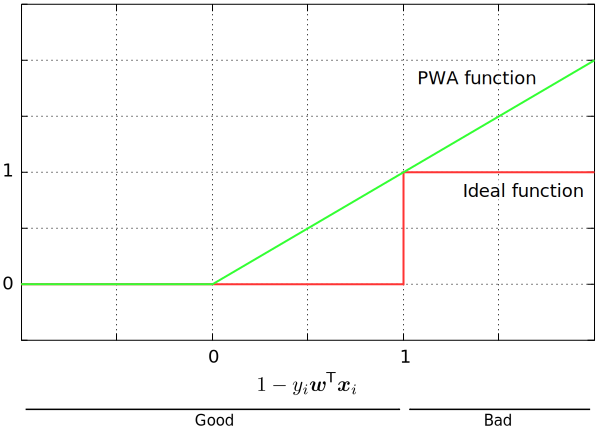
\includegraphics[clip,width=240pt]{figures/eval_curve_2.pdf}}
\caption{理想的なペナルティ関数とSVMで使われるペナルティ関数}
\label{fig:eval_curve_2}
\end{figure}


\subsection{サポートベクターマシンの定式化}

図\ref{fig:eval_curve_2}における区分的アファイン関数を$V_{\mathrm{svm}}$とおくとしよう.
このときSVMは
\begin{align}
    \label{eqn:svm_1}
    y &= \Sgn \left( \bs{w}\tran\bs{x} \right), \\
    \label{eqn:svm_2}
    \bs{w} &= \argmin_{\bs{w}} \sum_{i \in \mathcal{I}} V_{\mathrm{svm}}
    \left( 1 - y_i \bs{w}\tran\bs{x}_i \right),
\end{align}
と定式化される.以下,最適化問題(\ref{eqn:svm_2})が線形計画問題
\begin{equation}\begin{split}
    \label{eqn:lp}
    \min_{\bs{p}} \hspace{6pt}& \bs{c}\tran\bs{p}, \\
    \text{s.t.}   \hspace{6pt}& \bs{A}\bs{p} \geq \bs{b},
\end{split}\end{equation}
に帰着されることを示す.
ペナルティ関数$V_{\mathrm{svm}} \left( 1 - y_i \bs{w}\tran\bs{x}_i \right)$
の値を$\xi_i$とおくと,
$\xi_i = V_{\mathrm{svm}} \left( 1 - y_i \bs{w}\tran\bs{x}_i \right)$は
\begin{equation}\begin{split}
    \min_{\xi_i} \hspace{6pt}& \xi_i,                                  \\
    \text{s.t.}  \hspace{6pt}& \xi_i \geq 1 - y_i \bs{w}\tran\bs{x}_i, \\
                             & \xi_i \geq 0,
\end{split}\end{equation}
と等価である.
これはSVMに限らず区分的アファイン関数の最適化で頻繁に利用されるテクニックである.    
したがって最適化問題(\ref{eqn:svm_2})は
\begin{equation}\begin{split}
    \min_{\xi_i, i \in \mathcal{I}} \hspace{6pt}& \sum_{i \in \mathcal{I}} \xi_i, \\
    \text{s.t.} \hspace{6pt}
    & \xi_i \geq 1 - y_i \bs{x}_i\tran\bs{w}, \hspace{10pt} \text{for all $i \in \mathcal{I}$}, \\
    & \xi_i \geq 0,                           \hspace{50pt} \text{for all $i \in \mathcal{I}$},
\end{split}\end{equation}
と変形できる.さらにここで
\begin{equation}
    \bs{\xi} \triangleq
    \begin{pmatrix}
        \xi_1  \\ \vdots \\ \xi_n
    \end{pmatrix},
    \hspace{5pt}
    \bs{p} \triangleq
    \begin{pmatrix}
        \bs{w} \\ \bs{\xi}
    \end{pmatrix},
    \hspace{5pt}
    \bs{Q} \triangleq
    \begin{pmatrix}
        y_1 \bs{x}_1\tran \\
        \vdots            \\
        y_n \bs{x}_n\tran \\
    \end{pmatrix},
\end{equation}
\begin{equation}
    \bs{A} \triangleq
    \begin{pmatrix}
        \bs{Q}        & \bs{I}_n \\
        \bs{O}_{n, m} & \bs{I}_n
    \end{pmatrix},
    \hspace{5pt}
    \bs{b} \triangleq
    \begin{pmatrix}
        \bs{1}_n \\ \bs{0}_n
    \end{pmatrix},
    \hspace{5pt}
    \bs{c} \triangleq
    \begin{pmatrix}
        \bs{0}_m \\ \bs{1}_n
    \end{pmatrix},
\end{equation}
とおけば,式(\ref{eqn:lp})に帰着される.
ただし$\bs{0}_\alpha$は$\alpha$次元の零ベクトル,
$\bs{1}_\alpha$はすべての要素が1の$\alpha$次元ベクトル,
$\bs{I}_\alpha$は$\alpha$次元の単位行列,
$\bs{O}_{\alpha, \beta}$は$\alpha \times \beta$次元の零行列である.


\subsection{線形サポートベクターマシンのPython実装}

線形SVMの実装としてはC/C++で実装されたLIBSVM
\footnote{\texttt{https://www.csie.ntu.edu.tw/\~{}cjlin/libsvm/}}
やLIBLINEAR
\footnote{\texttt{https://www.csie.ntu.edu.tw/\~{}cjlin/liblinear/}}
が有名である.またこれらをPythonから統一的なインタフェースで呼び出すことの出来るライブラリとして
scikit-learn
\footnote{\texttt{https://scikit-learn.org/stable/}}
がある.応用上はこれらのパッケージを使うのが現実的であるが,
試みに前節で紹介した定式化をPythonで実装したものを本文書と同じレポジトリに同梱してある.
必要に応じて参考にして頂きたい.
ただし線形計画問題を解くパッケージとしてPulpを,グラフの描画にMatplotlibを使用した.
これらのパッケージは以下のコマンドでインストールできる.

\begin{center}
\verb|$ pip3 install pulp matplotlib|
\end{center}


%%%%%%%%%%%%%%%%%%%%%%%%%%%%%%%%%%%% SOURCE FINISH %%%%%%%%%%%%%%%%%%%%%%%%%%%%%%%%%%
% vim: expandtab shiftwidth=4 tabstop=4 filetype=tex
